%% 
%% Copyright 2007-2025 Elsevier Ltd
%% 
%% This file is part of the 'Elsarticle Bundle'.
%% ---------------------------------------------
%% 
%% It may be distributed under the conditions of the LaTeX Project Public
%% License, either version 1.3 of this license or (at your option) any
%% later version.  The latest version of this license is in
%%    http://www.latex-project.org/lppl.txt
%% and version 1.3 or later is part of all distributions of LaTeX
%% version 1999/12/01 or later.
%% 
%% The list of all files belonging to the 'Elsarticle Bundle' is
%% given in the file `manifest.txt'.
%% 
%% Template article for Elsevier's document class `elsarticle'
%% with numbered style bibliographic references
%% SP 2008/03/01
%% $Id: elsarticle-template-num.tex 272 2025-01-09 17:36:26Z rishi $
%%
\documentclass[preprint,12pt]{elsarticle}

%% Use the option review to obtain double line spacing
%% \documentclass[authoryear,preprint,review,12pt]{elsarticle}

%% Use the options 1p,twocolumn; 3p; 3p,twocolumn; 5p; or 5p,twocolumn
%% for a journal layout:
%% \documentclass[final,1p,times]{elsarticle}
%% \documentclass[final,1p,times,twocolumn]{elsarticle}
%% \documentclass[final,3p,times]{elsarticle}
%% \documentclass[final,3p,times,twocolumn]{elsarticle}
%% \documentclass[final,5p,times]{elsarticle}
%% \documentclass[final,5p,times,twocolumn]{elsarticle}

%% For including figures, graphicx.sty has been loaded in
%% elsarticle.cls. If you prefer to use the old commands
%% please give \usepackage{epsfig}

% The preceding line is only needed to identify funding in the first footnote. If that is unneeded, please comment it out.
\usepackage{cite}
\usepackage{url}
%\usepackage{algorithmic}
\usepackage{textcomp}
\usepackage[font=footnotesize]{caption}
%\newcommand{\captionsize}{\fontsize{8pt}{1.18em}\selectfont}




\let\proof\relax \let\endproof\relax
\usepackage[font=scriptsize]{caption}

\newcommand\qedsymbol{$\blacksquare$}
%\usepackage{graphicx}
%\usepackage{breqn}
%\usepackage{array, mathtools}
%\usepackage{siunitx}
% \usepackage[ruled,vlined]{algorithm2e}
\usepackage{algorithm}
\usepackage[noend]{algpseudocode}
\algnewcommand\algorithmicKwIn{\textbf{Input: }}
\algnewcommand\algorithmicKwOut{\textbf{Output: }}
\algnewcommand\algorithmicKwData{\textbf{Data: }}
\algnewcommand\algorithmicKwInit{\textbf{Initialize }}
\algnewcommand\algorithmicKwConstruct{\textbf{Construct }}
\algnewcommand\algorithmicKwCalculate{\textbf{Calculate }}
\algnewcommand\algorithmicKwReturn{\textbf{Return }}

\usepackage{tabulary}
\usepackage{color}
\usepackage{tikz, pgfplots}
\usepackage{graphicx}
\usepackage{tabularx}
\usepackage{amsmath, amssymb, amssymb, amsthm}

\usepackage{mathtools}
%\mathtoolsset{showonlyrefs}

\newcommand{\D}{\mathcal{D}}
\renewcommand{\SS}{\texttt{S}}
\newcommand{\CC}{\texttt{C}}
\newcommand{\ul}{\underline}
\newcommand{\tcr}{\textcolor{red}}
\newcommand{\mc}{\mathcal}
\newcommand{\ov}{\overline}
\newtheorem{prop}{Proposition}
\newtheorem{theorem}{Theorem}
\newtheorem{fact}{Fact}
\newtheorem{lemma}{Lemma}
\newtheorem{observation}{Observation}
\newtheorem{assumption}{Assumption}
\newtheorem{problem}{Problem}
\newtheorem*{remark}{Remark}

\usepackage{comment}
\usepackage{caption}

\usetikzlibrary{calc,shapes.callouts,shapes.arrows}
\usetikzlibrary{arrows,arrows.meta,automata,shapes,calc,intersections}
\usepgfplotslibrary{fillbetween}
\pgfplotsset{compat=newest}
\usetikzlibrary{calc}
\usetikzlibrary{positioning}
%\usetikzlibrary{intersections}
\usepackage{caption}
\usepackage{subcaption}

\usetikzlibrary{external}
% \tikzexternalize[prefix=tikz/]
\usepgfplotslibrary{external} 
% \tikzexternalize


\definecolor{mycolor1}{RGB}{230,97,1}
\definecolor{mblue}{rgb}{0.176, 0.380, 0.659}
\newcommand{\Xsafe}{\mathcal{X}_{\textnormal{safe}}}
\newcommand{\Xunsafe}{\mathcal{X}_{\textnormal{unsafe}}}
\newcommand{\Xgoal}{\mathcal{X}_{\textnormal{goal}}}
\usepackage{acronym}
\acrodef{GP}[GP]{Gaussian Process}

\acrodef{MPC}[MPC]{Model Predictive Control}

\DeclareMathOperator*{\argmin}{argmin}
\newcommand{\ol}{\overline}
\captionsetup[figure]{font=normalsize,labelfont=normalsize}

\journal{Nonlinear Analysis: Hypbrid Systems}
\begin{document}

\begin{frontmatter}
\title{\LARGE \bf Trajectory Tracking for Systems with Unknown Time-Varying Disturbances}
\author{Michael E. Cao, Akash Harapanahalli, Evanns Morales-Cuadrado(?), and Samuel Coogan% <-this % stops a space
\thanks{M. E. Cao, A. Harapanahalli, E. Morales-Cuadrado, and S. Coogan are with the School of Electrical and Computer Engineering, Georgia Institute of Technology, Atlanta, 30332, USA {\tt\small \{mcao34, aharapan, egm, sam.coogan\}@gatech.edu}. S. Coogan is also with the School of Civil and Environmental Engineering, Georgia Institute of Technology, Atlanta, 30332, USA.
This work was supported in part by the National Science Foundation under awards \#1749357 and \#1924978, and the NASA University Leadership Initiative under grant \#80NSSC20M0161. This article solely reflects the opinions and conclusions of its authors.
}
}



% \maketitle


% \thispagestyle{empty}
% \pagestyles{empty}


%%%%%%%%%%%%%%%%%%%%%%%%%%%%%%%%%%%%%%%%%%%%%%%%%%%%%%%%%%%%%%%%%%%%%%%%%%%%%%%%
\begin{abstract}

We consider nonlinear systems with partially unknown time-dependent and state-dependent dynamics. Given a reference trajectory, we leverage the mixed monotonicity property of dynamical systems to develop a formulation that efficiently calculates a forward invariant tube around said trajectory. This efficiency comes from the creation of an embedding system, a single trajectory of which produces the forward invariant tube. We incorporate the unknown portions of the dynamics by modeling them as time-varying Gaussian processes, and develop a general mixed-Jacobian-based embedding system that accounts for the first order interactions between the disturbance behavior, feedback controller, and system state. We demonstrate the efficacy of this formulation in a direct trajectory tracking scenario as well as part of an implicit active set invariance filter over a separate controller.

\end{abstract}

\end{frontmatter}
%%%%%%%%%%%%%%%%%%%%%%%%%%%%%%%%%%%%%%%%%%%%%%%%%%%%%%%%%%%%%%%%%%%%%%%%%%%%%%%%
\section{Introduction}
\label{section:introduction}
Safety-critical autonomous systems often require guarantees that they will only operate within an allowable safe region of their statespace.
As a motivating example considered throughout this paper, in the context of urban air mobility, one key safety requirement is the ability of aerial vehicles to land without damaging the vehicle or the environment around it. As these vehicles are operating in uncontrolled outdoor environments, they are subject to environmental disturbances that are not known a priori. While techniques exist for planning trajectories that are nominally safe~\cite{heidari2021trajectory}, 
% ensuring that the system is able to track these trajectories during runtime in the presence of unknown disturbances is challenging. The goal of this work is to design a runtime-assurance framework that ensures safety  in the presence of unknown disturbances. Our approach is to compute forward invariant tubes for the system given the limits of the control input and the current knowledge of the disturbance behavior, and override a nominal tracking control law if the system is at risk of violating its safety restrictions.
the presence of unknown disturbances in the environment means that precise tracking of these trajectories is a challenge. Thus, the goal of this work is to derive a formulation that calculates a forward invariant tube around the reference trajectory that accounts for the unknown disturbance behavior. This formulation can then enforce accurate tracking of said reference trajectory.

In many cases, uncertainty in the dynamics can be learned via observations. For example, the position-dependent wind field that an aerial vehicle encounters might be unknown a priori but can be learned through observations of the wind at different points. 
For such systems, in~\cite{caoMMGPs, caoMMGPOJCSYS}, we derive high probability bounds on the unknown disturbance behavior by modeling the disturbance as a state-dependent Gaussian Process (GP). In turn, these bounds enable us to calculate overapproximations of the reachable sets of the system that hold with high probability. For this, we leverage the \emph{mixed monotonicity} property of dynamical systems to embed the dynamics in a higher dimensional system~\cite{cooganMixMono, ENCISO2006205}. A key advantage of this overapproximation technique is its computational efficiency: it reduces the reachable set computation to the evaluation of a single trajectory of an \emph{embedding system} with twice the number of states as the original system. This computation is able to be updated in real-time, even for systems of moderately high dimension~\cite{abate2021hscc}, and we leverage this property in~\cite{caoICRARTA} to develop an approach that dynamically detects when a new observation of the disturbance behavior needs to be collected to keep the system within an acceptable bound of the reference trajectory. It then updates the reference trajectory and forward invariant tube with the new observation during runtime to preserve safety. However, this approach requires several limiting assumptions on the system dynamics and does not consider potentially time-varying disturbance behaviors. Thus, the focus of this work is on generalizing this technique to a wider array of dynamical systems and to account for time-varying disturbances.

There are several methods for ensuring safety at runtime, which is commonly referred to as runtime assurance. The most common runtime assurance architecture is the Simplex architecture proposed by~\cite{sha2001}, where two controllers are developed for the system: one that is high-assurance and another that is high-performance. The high-performance controller is allowed to run until some predetermined decision logic detects that the system is about to violate a safety specification, at which point control is switched to the high-assurance controller. This allows the high-performance controller to be developed without having to validate that it is safe beforehand. Alternatively,~\cite{gurriet2018} introduces online active set invariance filtering, which instead minimally modifies the control action such that there exists a back-up trajectory that takes the system to a safe set, while never actually needing to execute the backup strategy. Another approach is introduced in~\cite{lee1999runtime}, which develops a formal language to implement runtime assurance. An illustrative example of practical runtime assurance for unmanned aerial systems is implemented in~\cite{schierman2020runtime}, though that method is implemented at the waypoint and trajectory selection level.

With regards to assurance for systems with partially unknown dynamics,~\cite{XiongNeural} develops a Twin Neural Lyapunov Function which is then used to build a runtime monitor. However, like many neural network applications, a large amount of training data is needed to ensure safety, and the formulation assumes no prior knowledge of the system's dynamics. Alternatively,~\cite{ghoriDist} develops a runtime assurance mechanism for distributed avionics architecture which can intervene in the event of failure. \cite{tarokhManip} develops a nested control strategy consisting of an outer task-space loop and an inner joint-space loop for the trajectory tracking problem on a manipulator with uncertain kinematics and dynamics.

Other approaches to the invariant tube synthesis problem (also known as the \emph{funnel synthesis} problem) include~\cite{BehcetFunnel}, which develops a funnel synthesis algorithm for computing controlled invariant sets around a given nominal trajectory by solving a differential LMI,~\cite{TOBENKINSoS} which develops several strategies utilizing Sum-of-Squares programming for computing regions of finite-time invariance around solutions of polynomial differential equations, and~\cite{FejlekFalsifier} which proposes an approach to funnel synthesis that is based on falsification. Additionally, \cite{kim2023joint} develops a joint trajectory and funnel synthesis technique for discrete-time systems with locally Lipschitz nonlinearities. Finally,~\cite{Reynolds6DOF, MajumdarRealTime} develop funnel synthesis strategies applied in real-time on aerial vehicles.

\cite{sivaramStochasticReach}

In this work, we leverage the mixed monotonicity property to derive a runtime assurance mechanism that can detect whether the controller is unable to follow the reference trajectory within a desired tolerance. Specifically, we apply the formulation proposed by~\cite{GirardAbstraction} to calculate a forward-invariant tube around the reference trajectory based on the current observations of the unknown disturbance behavior and the limits of the controller, and we then design a controller which guarantees this forward invariance. Next, we define a safe deviation threshold which, if crossed, triggers an observation of the unknown dynamics and a recalculation of the reference trajectory and forward invariant tube, ensuring that the system never deviates from the reference trajectory by more than the safe threshold. We demonstrate this formulation on a case study of a planar multirotor vehicle making a safe landing in a wind field.

In contrast to the current literature, our proposed formulation natively accommodates nonlinear dynamics without the need to solve for LMIs, which are relatively expensive computationally. Additionally, we solve the problem fully in continuous-time and do not need to choose time discretization points. Finally, we propose a method for sampling to improve knowledge of the unknown dynamics that minimizes the number of samples needed to ensure safety.

We build upon previous work~\cite{caoICRARTA}, which focused on developing a runtime assurance mechanism for trajectory tracking for systems with unknown time-invariant disturbance behavior. We expand upon this work by introducing a mixed Jacobian method for constructing a general embedding system that produces a high-probability forward invariant tube around the reference trajectory without an interval assumption on the dynamics, incorporating time-varying disturbance behaviors into the formulation, and showcasing the formulation on physical hardware.

The rest of this paper is structured as follows: 
we introduce key notation in Section~\ref{section:notation}, define our problem in Section~\ref{section:problem}, and provide key preliminaries in~\ref{section:prelim}. We then derive our forward-invariant tube formulation and runtime assurance mechanism in Section~\ref{section:finv}, and apply it to case studies of a planar multirotor vehicle in Section~\ref{section:sim}. We conclude with a discussion in Section~\ref{section:conclusion}.

\section{Notation}
\label{section:notation}
Let $(x, y)$ denote the vector concatenation of $x, y \in \mathbb{R}^n$, i.e., $(x, y) := [x^T\ y^T]^T \in \mathbb{R}^{2n}$. Additionally, $\preceq$ denotes the componentwise vector order, i.e., $x\preceq y$ if and only if $x_i \leq y_i$ for all $i\in\{1, ..., n\}$ where vector components are indexed via subscript.

Given $x,y \in \mathbb{R}^n$ such that $x\preceq y$, we denote the hyperrectangle defined by the endpoints $x$ and $y$ using the notation
 $   [x, y]:=\{z\in\mathbb{R}^n\ |\ x\preceq z\text{ and }z\preceq y\}.
 $ 
Also, given $a = (x, y)\in\mathbb{R}^{2n}$ with $x\preceq y$, $[\![a]\!]$ denotes the hyperrectangle formed by the first and last $n$ components of $a$, i.e., $[\![a]\!] := [x, y]$. Finally, let $\preceq_\text{SE}$ denote the \textit{southeast order} on $\mathbb{R}^{2n}$ defined by $(x, x')\preceq_\text{SE}(y, y')$ if and only if $x\preceq y \text{ and } y'\preceq x'$. In particular, observe that when $x\preceq x'$ and $y\preceq y'$, 
\begin{equation}
\label{eq:box}
    (x, x')\preceq_\text{SE}(y, y') \iff [y, y']\subseteq[x, x'].
\end{equation}
Finally, $x_{[i:y]}$ denotes the vector $x$ whose $i$th component has been replaced with the $i$th component of vector $y$.

\section{Problem Setup}
\label{section:problem}
We consider the continuous-time, nonlinear, Lipschitz-continuous system
\begin{equation}
    \dot{x} = f(x, u, w)
    \label{eq:system}
\end{equation}
where $x \in \mathbb{R}^n$ is the system state, 
% $u \in U = [\ul{u}, \ol{u}] \subset \mathbb{R}^m$ 
$u \in \mathbb{R}^m$ 
is the system input,
%constrained to an interval,
and $w \in \mathbb{R}^p$ is an unknown, time-varying, state-dependent component of the dynamics so that $w_i=g_i(t, x)$ where $g_i$ is unknown. 

% We make the following smoothness assumption on the behavior of $g(t, x)$.

Given a set of reference trajectories, our objective is to efficiently compute a forward invariant tube around said reference trajectories that holds with high probability. Thus, we formally define our problem as follows.

\begin{problem}
Given a system~\eqref{eq:system} and reference trajectories $x_r, u_r$, produce a controlled forward-invariant tube around the reference trajectory that holds with probability at least $1-\eta$.
\label{prob}
\end{problem}

Multiple formulations exist to produce safe trajectories for, \emph{e.g.},  autonomous aerial vehicles, leveraging techniques from optimal control~\cite{heidari2021trajectory, HEHNtraj}, and differential flatness~\cite{murray1995differential, ChamseddineQuadrotor}, for example.
In this work, we are specifically interested in the problem of calculating a forward invariant tube around the given reference trajectory in the presence of unknown disturbance behavior at runtime. Thus, we presume that any of these techniques are readily available for generating the reference trajectory.

\section{Preliminaries}
\label{section:prelim}
In this section, we provide an overview of mixed monotonicity and how it enables efficient calculation of reachable set overapproximations. We then illustrate how the introduction of Gaussian Processes (GPs) leads to overapproximations of reachable sets that hold with high probability. This formulation will be modified in subsequent sections to produce our forward invariant tube around a reference trajectory.

\subsection{Mixed Monotonicity}
The system~\eqref{eq:system} is \emph{mixed monotone with respect to a decomposition function $\delta$} if $\delta$ satisfies the following:
\begin{enumerate}
    \item For all $x, u, w$, 
    \begin{equation}
        \delta (x, u, w, x, u, w) = f(x, u, w)
    \end{equation}
    \item For all $x \preceq \widehat{x}$, $u \preceq \widehat{u}$, $w \preceq \widehat{w}$, and all $a \in [x, \widehat{x}]$, $b \in [u, \widehat{u}]$, $c \in [w, \widehat{w}]$,
    \begin{equation}
        \delta (x, u, w, \widehat{x}, \widehat{u}, \widehat{w}) \preceq f(a, b, c) \preceq \delta ( \widehat{x}, \widehat{u},\widehat{w}, x, u, w)
    \end{equation}
    \item For all $i\in \{1,...,n\}$,
    \begin{equation}
         \delta_i (x, u, w, \widehat{x}, \widehat{u}, \widehat{w})\leq\delta_i (x', u', w', \widehat{x}', \widehat{u}', \widehat{w}')
    \end{equation}
    for all $(x, \widehat{x})\preceq_\text{SE}(x', \widehat{x}')$ such that $x_i = x'_i$, $(u, \widehat{u})\preceq_\text{SE}(u', \widehat{u}')$, $(w, \widehat{w})\preceq_\text{SE}(w', \widehat{w}')$
\end{enumerate}
Additionally, $\delta$ is said to be \emph{tight} if it is such that
\begin{align}
    \delta_i(\ul{x}, u, w, \ol{x}, \widehat{u}, \widehat{w}) &= \min_{a \in [\ul{x}, \ol{x}], a_i = \ul{x}_i}\min_{b \in [u, \widehat{u}]}\min_{c \in [w, \widehat{w}]} f_i(a, b, c) \label{eq:tight1}\\
    \delta_i(\ol{x}, \widehat{u}, \widehat{w}, \ul{x}, u, w) &= \max_{a \in [\ul{x}, \ol{x}], a_i = \ul{x}_i}\max_{b \in [u, \widehat{u}]}\max_{c \in [w, \widehat{w}]} f_i(a, b, c).\label{eq:tight2}
\end{align}

For any system, there exists some decomposition function $\delta$ satisfying the above conditions~\cite{abateTight}, although one may not be readily available in closed form. For more examples of decomposition functions and practical applications of mixed monotonicity, see~\cite{caoMMGPsMPC, abateSpaceCraft}.

Given mixed monotone system \eqref{eq:system} and a corresponding decomposition function, we then construct the \emph{embedding system} with state $(\ul{x}, \ol{x}) \in \mathbb{R}^n\times \mathbb{R}^n$, input $(u,\widehat{u}) \in \mathbb{R}^m\times\mathbb{R}^m$, and disturbance $(w, \widehat{w}) \in \mathbb{R}^p \times \mathbb{R}^p$ defined by the dynamics
\begin{equation}
\label{eq:embed_init}
    \begin{bmatrix}
    \dot{\ul{x}} \\
    \dot{\ol{x}}
    \end{bmatrix} = \varepsilon(\ul{x}, u, w, \ol{x}, \widehat{u},\widehat{w}) :=
    \begin{bmatrix}
    \delta(\ul{x}, u, w, \ol{x}, \widehat{u},\widehat{w}) \\
    \delta(\ol{x}, \widehat{u}, \widehat{w}, \ul{x}, u, w)
    \end{bmatrix}.
\end{equation}
Denote the state of~\eqref{eq:system} at time $t$ when initialized at $x_0$ under some input signal $u:[0,\infty)\to\mathbb{R}^m$ and some disturbance signal $w:[0,\infty)\to\mathbb{R}^p$ by $\phi(t; x_0, u, w)$, and denote the state of~\eqref{eq:embed_init} at time $t$ initialized at $(\ul{x}_0,\ol{x}_0)$ under some input signal $(u, \widehat{u}):[0,\infty)\to\mathbb{R}^m\times\mathbb{R}^m$, and disturbance signal $(w,\widehat{w}):[0,\infty)\to\mathbb{R}^p\times \mathbb{R}^p$ by $\Phi^\varepsilon(t;(\ul{x}_0, \ol{x}_0), (u,\widehat{u}), (w, \widehat{w}))$. The fundamental result of mixed monotone systems theory is that~\eqref{eq:embed_init} is a monotone control system as defined in \cite{angeliMonotone} with respect to the southeast order on state, input, and disturbance; that is, given $a, a' \in \mathbb{R}^n\times \mathbb{R}^n$, $b, b':[0, \infty) \rightarrow \mathbb{R}^m\times\mathbb{R}^m$ and $c, c':[0, \infty) \rightarrow \mathbb{R}^p\times \mathbb{R}^p$ such that $a \preceq_\text{SE} a'$, $b \preceq_\text{SE} b'$, and $c(t) \preceq_\text{SE} c'(t)$ for all $t\geq0$, then for all $t\geq0$,
\begin{equation}
    \Phi^\varepsilon(t; a, b, c) \preceq_\text{SE} \Phi^\varepsilon(t; a', b', c').
    \label{eq:monotone_system}
\end{equation}
In other words, provided that the system is initialized within $[\ul{x}_0, \ol{x}_0]$, the input signal is overapproximated by $[u, \widehat{u}]$, and the disturbance signal is overapproximated by $[w, \widehat{w}]$, then the hyperrectangle defined by $[\![\Phi^\varepsilon(t;(\ul{x}_0, \ol{x}_0), (u,\widehat{u}), (w, \widehat{w}))]\!]$ overapproximates the true reachable set 
of~\eqref{eq:system}, \emph{i.e.}
\begin{equation}
    \phi(T; x_0, u, w) \subseteq [\![\Phi^\varepsilon(T;(\ul{x}_0, \ol{x}_0), (u,\widehat{u}), (w, \widehat{w}))]\!]
\end{equation}
for all $T \geq 0$ and $x_0 \in [\ul{x}_0, \ol{x}_0]$.

\subsection{Gaussian Processes and High Probability Reachable Sets}
\label{section:gp}
If there exist known bounding functions $\ul{\gamma}_i(t, \ul{x}, \ol{x})$ and $\ol{\gamma}_i(t, \ul{x}, \ol{x})$, $\ul{\gamma}_i, \ol{\gamma}_i: \mathbb{R} \times \mathbb{R}^n\times\mathbb{R}^n\mapsto\mathbb{R}$, for all $i\in\{1,\ldots,p\}$ such that 
\begin{equation}
\label{eq:GPbound}
    \ul{\gamma}_i(t, \ul{x},\ol{x}) \leq g_i(t, x) \leq \ol{\gamma}_i(t, \ul{x}, \ol{x}), x \in [\ul{x}, \ol{x}], 
\end{equation}
for all $t$ and all $\ul{x}, \ol{x}\in\mathbb{R}^n$ with $\ul{x}\preceq \ol{x}$, where $g(t, x)$ represents the a priori unknown function dictating the behavior of $w$, then these functions can be inserted into the previously described embedding system to produce valid reachable set overapproximations. This is achieved by taking the embedding system~\eqref{eq:embed_init} and inserting $\ul{\gamma}(t, \ul{x},\ol{x}), \ol{\gamma}(t, \ul{x},\ol{x})$ in place of $w, \widehat{w}$ to produce a new embedding system as
\begin{equation}
\label{eq:emb1}
    \begin{bmatrix}
    \dot{\ul{x}} \\
    \dot{\ol{x}}
    \end{bmatrix} = e(t, \ul{x}, u, \ol{x}, \widehat{u}) :=
    \begin{bmatrix}
    \delta(\ul{x}, u, \ul{\gamma}(t, \ul{x}, \ol{x}), \ol{x},  \widehat{u}, \ol{\gamma}(t, \ul{x}, \ol{x})) \\
    \delta(\ol{x},  \widehat{u}, \ol{\gamma}(t, \ul{x}, \ol{x}), \ul{x},  u, \ul{\gamma}(t, \ul{x}, \ol{x}))
    \end{bmatrix}.
\end{equation}


We have shown previously in~\cite{caoMMGPOJCSYS} that for time-invariant disturbance functions $g_i(x)$, modeling these functions as GPs enables the formulation of bounding functions that fulfill the time-invariant version of~\eqref{eq:GPbound} with probability $1-\eta, \eta\in(0, 1]$. We now extend these results to the time-varying setting and derive bounds that fulfill~\eqref{eq:GPbound} with probability $1-\eta$.

We pull from~\cite{bogunovicTVGP} and model $g$ using a \ac{GP} with a spatiotemporal kernel model with temporal kernel of the form
\begin{equation}
    (1-\epsilon)^\frac{|t_1-t_2|}{2}
    \label{eq:time_kernel}
\end{equation}
where $\epsilon \in [0, 1]$ represents the rate of change in $g$ over time. $\epsilon=1$ recovers the time-invariant model of $g$, while $\epsilon = 0$ means that the behavior of $g$ is entirely independent between any two observation times.

We first review the standard time-invariant model. Given a set of $\tau$ observations $\{y_j\}_{j=1}^\tau$ of the \ac{GP} at corresponding points $\{x_j\}_{j=1}^\tau$, the surrogate functions of interest to approximate $g_i$ are 
\begin{align}
    \forall i\in\{1,\cdots,p\}, \quad
    \begin{cases}
    \ol{g}_{i}^{(\tau)}(x) := \mu_\tau(x) + \sqrt{\beta_\tau}\sigma_{\tau}(x)\\
    \ul{g}_i^{(\tau)}(x) := \mu_\tau(x) - \sqrt{\beta_\tau}\sigma_{\tau}(x)\\
    \end{cases}\label{eq:GP-UCB}
\end{align}
where $\beta_\tau$ is chosen as per~\cite[Theorem 7]{caoMMGPOJCSYS},
% \begin{align}
%     \beta_t := 2 \log\left(\frac{pt^2\pi^2}{3\eta}\right) + 2n \log\left(t^2nbr\sqrt{\log\left(\frac{2pna}{\eta}\right)}\right),
% \end{align}
$\mu_\tau(\cdot)$ is the posterior mean, and $\sigma_\tau(\cdot)$ is the posterior variance, computed according to the standard \ac{GP} updates~\cite{Rasmussen2006}:
\begin{align}
    \mu_\tau(x) &:= k_\tau(x)^T(K_\tau+\sigma^2 I)^{-1}y_\tau\\
    k_\tau(x,x') &:= k(x,x')-k_\tau(x)^T(K_\tau+\sigma^2 I)^{-1}k_\tau(x')\\
    \sigma_\tau^2(x) &:= k_\tau(x,x)
\end{align}
where $k_\tau(x):= (k(x_1,x),\cdots,k(x_\tau,x))$ and $K_\tau=\left[k_\tau(x_i,x_j)\right]$. To extend this formulation into the time-varying case, we now leverage that the observations $\{y_j\}_{j=1}^\tau$ are taken at times $\{t_j\}_{j=1}^\tau$. Given temporal kernel~\eqref{eq:time_kernel}, the updated posterior mean and variance equations for querying a point at time $t_{\tau + 1}$ are
\begin{align}
    \widetilde{\mu}_{\tau+1}(x) &:= \widetilde{k}_\tau(x)^T(\widetilde{K}_\tau+\sigma^2 I)^{-1}y \label{eq:tvmean}\\
    k_{\tau+1}(x,x') &:= k(x,x')-\widetilde{k}_\tau(x)^T(\widetilde{K}_\tau+\sigma^2 I)^{-1}\widetilde{k}_\tau(x')\\
    \widetilde{\sigma}_{\tau+1}^2(x) &:= k_{\tau+1}(x,x) \label{eq:tvsig}
\end{align}
with
\begin{align}
    \widetilde{K}_\tau &= K_\tau \odot [(1 - \epsilon)^{|t_i - t_j|/2}]_{i,j=1}^\tau \\
    \widetilde{k}_\tau(x) &= k_\tau(x) \odot [(1-\epsilon)^{(t_{\tau+1} - t_i)/2}]_{i=1}^\tau
\end{align}
where $\odot$ is the Hadamard product. Thus, the surrogate functions of interest to approximate time-varying $g_i$ are 
\begin{align}
    \forall i\in\{1,\cdots,p\}, \quad
    \begin{cases}
    \ol{g}_{i}^{(\tau + 1)}(x) := \widetilde{\mu}_{\tau+1}(x) + \sqrt{\beta_\tau}\widetilde{\sigma}_{\tau+1}(x)\\
    \ul{g}_i^{(\tau + 1)}(x) := \widetilde{\mu}_{\tau+1}(x) - \sqrt{\beta_\tau}\widetilde{\sigma}_{\tau+1}(x)\\
    \end{cases}\label{eq:TVGP-UCB}
\end{align}
Then, for all $i\in\{1,\cdots,p\}$ and all $\tau\geq 1$, define for all $\underline{x}\preceq \overline{x}$,
\begin{align}
\underline{\gamma}_i(\tau + 1, \underline{x},\overline{x}) &:= \min_{x\in[\underline{x}^{(\tau,-)},\overline{x}^{(\tau,+)}]\cap \mathcal{D}_\tau} \underline{g}^{(\tau + 1)}_i(x)-\frac{1}{(\tau+1)^2},\label{eq:surrogate_functions2a}\\
\overline{\gamma}_i(\tau+1, \underline{x},\overline{x}) &:= \max_{x\in[\underline{x}^{(\tau,-)},\overline{x}^{(\tau,+)}]\cap \mathcal{D}_\tau} \overline{g}^{(\tau + 1)}_i(x)+\frac{1}{(\tau+1)^2}.
\label{eq:surrogate_functions2b}
\end{align}
where $\underline{x}^{(\tau,-)},\overline{x}^{(\tau,+)}$ are defined as in~\cite[Equations 54-55]{caoMMGPOJCSYS}. These functions fulfill~\eqref{eq:GPbound} with probability at least $1-\eta$, and thus the reachable set overapproximations calculated by the embedding system~\eqref{eq:emb1} using these functions hold with probability at least $1-\eta$.

\section{Feedback Aware Forward Invariance}
\label{section:finv}
In this section, we develop a Jacobian-based general embedding system formulation for calculating a forward invariant tube around a reference trajectory. This new formulation incorporates a known feedback control strategy, allowing for the tube to be controlled forward invariant and thus enabling the runtime assurance mechanism to work on general nonlinear systems of the form~\eqref{eq:system}.

We first introduce the mixed Jacobian operator, which is defined as follows. Given some $x \in \mathbb{R}_a$ and a differentiable function $f:\mathbb{R}^a\rightarrow\mathbb{R}^b$, define the mixed Jacobian operator $M_{x'}$ such that $M_{x'}f:\mathbb{R}^a \times [0, 1]^a \rightarrow \mathbb{R}^{a\times b}$ where
\begin{align}
    &(M_{x'}f(x, s))_{ij} =  \nonumber\\
    &\frac{\partial f_i}{\partial x_j}(x_1, ..., x_{j-1}, s_jx_j + (1-s_j)x'_j, x'_{j+1}, ..., x'_a)
\end{align}
for all $i = 1, ..., b$ and $j = 1,...,a$. Given an interval set $X=X_1 \times ...\times X_b$ and some $x' \in X$, we define an interval matrix $[\mathcal{M}]$ that overapproximates the mixed Jacobian of~\eqref{eq:system} over $X$. In other words, $[\mathcal{M}]$ is such that
\begin{equation}
    (M_{x'}f(x, s))_{ij} \subseteq [\mathcal{M}]_{ij}
    \label{eq:mixed_req}
\end{equation}
for all $i = 1, ..., b$ and $j = 1,...,a$. Per~\cite[Corollary 1]{harapanahalliLDI}, this is fulfilled if
\begin{equation}
    \frac{\partial f_i}{\partial x_j}(X_1, ..., X_j, x'_{j+1}, ..., x'_a) \subseteq [\mathcal{M}]_{ij}
    \label{eq:mixed_interval}
\end{equation}
for all $i = 1, ..., b$ and $j = 1,...,a$. As a result, it must hold that
\begin{equation}
    f(x) - f(x') \in [\mathcal{M}](x - x').
\end{equation}

We expand~\eqref{eq:mixed_req} to fit systems of the form~\eqref{eq:system}. First, we define the interval sets $X=X_1 \times ...\times X_n$, $U=U_1 \times ...\times U_m$, $W=W_1 \times ...\times W_p$ as well as some $x' \in X$, $u' \in U$, and $w' \in W$. Thus,~\eqref{eq:mixed_req} becomes
\begin{equation}
    (M_{(x', u', w')}f(x, u, w, s))_{ij} \subseteq \begin{bmatrix}\mathcal{M}_x & \mathcal{M}_u & \mathcal{M}_w\end{bmatrix}_{ij}
\end{equation}
for all $i = 1, ..., n$ and $j = 1, ..., n+m+p$ over $X, U, W$. Applying~\eqref{eq:mixed_interval} results in this requirement being fulfilled if
\begin{align}
    &\frac{\partial f_i}{\partial x_j}(X_1, ..., X_j, x'_{j+1}, ..., x'_n, u'_1,...,u'_m, w'_1,...,w'_p) \nonumber \\
    &\subseteq [\mathcal{M}_x]_{ij}
\end{align}
for all $i,j = 1, ..., n$,
\begin{align}
    &\frac{\partial f_i}{\partial u_j}(X_1, ..., X_n,U_1, ..., U_j, u'_{j+1}, ..., u'_m, w'_1, ..., w'_p) \nonumber \\
    &\subseteq [\mathcal{M}_u]_{ij}
\end{align}
for all $i = 1, ..., n$, $j = 1, ..., m$, and
\begin{align}
    &\frac{\partial f_i}{\partial w_j}(X_1, ..., X_n, U_1, ..., U_m, W_1, ..., W_j, w'_{j+1}, ..., w'_p) \nonumber \\
    &\subseteq [\mathcal{M}_w]_{ij}
\end{align}
for all $i = 1, ..., n$, $j = 1, ..., p$. It consequently holds that
\begin{align}
    f(x, u, w) - f(x', u, w) &\in [\mathcal{M}_x](x - x'),
    \label{eq:Mx_diff} \\
    f(x, u, w) - f(x, u', w) &\in [\mathcal{M}_u](u - u'),
    \label{eq:Mu_diff} \\
    f(x, u, w) - f(x, u, w') &\in [\mathcal{M}_w](w - w').
    \label{eq:Mw_diff}
\end{align}
Thus, combining \eqref{eq:Mx_diff}, \eqref{eq:Mu_diff}, and \eqref{eq:Mw_diff} gives
\begin{align}
    f(x, u, w) - f(x', u', w') &\in  \\
    [\mathcal{M}_x](x - x') + [\mathcal{M}_u]&(u - u') + [\mathcal{M}_w](w - w'). \nonumber
\end{align}

As a result, given interval sets $X:=[x, \widehat{x}], U:=[\ul{u}, \ol{u}], W:=[\ul{w}, \ol{w}]$, and reference trajectories $x_r, u_r, w_r$ initialized within $X, U, W$, we formulate generalized embedding system dynamics for~\eqref{eq:system} as
\begin{align}
    [\dot{x}, \dot{\widehat{x}}] := &[\mathcal{M}_x]([x, \widehat{x}] - x_r) + [\mathcal{M}_u]([\ul{u}, \ol{u}] - u_r) \\
    &+ [\mathcal{M}_w]([\ul{w}, \ol{w}] - w_r) + f(x_r, u_r, w_r). \nonumber
\end{align}
\subsection{Feedback Controller Synthesis}
We then synthesize 
\begin{equation}
    [\mathcal{M}_x] + [\mathcal{M}_w][\mathcal{M}_g]
\end{equation}

\begin{equation}
    \begin{bmatrix}
        AQ+QA^T+BY+Y^TB^T & (CQ+DY)^T\\
        CQ+DY & -I
    \end{bmatrix} < 0
\end{equation}
\begin{equation}
    K = YQ^{-1}
\end{equation}
\subsection{Incorporation of First-Order Interactions}
Since we are attempting to track a reference trajectory, we incorporate a known feedback control strategy into our forward invariant tube calculation. We consider a feedback controller of the form 
\begin{equation}
\label{eq:feedback_controller}
    u = K(x - x_r) + u_r
\end{equation}
which, when inserted into the generalized embedding system, results in dynamics
\begin{align}
    [\dot{x}, \dot{\widehat{x}}] := &([\mathcal{M}_x] + K[\mathcal{M}_u])([x, \widehat{x}] - x_r) \label{eq:gen_emb}\\
    &+ [\mathcal{M}_w]([w, \widehat{w}] - w_r) + f(x_r, u_r, w_r).\nonumber
\end{align}
The above embedding system produces a valid forward invariant tube around the reference trajectory %  and the gamma bounds and mean behavior can be inserted to produce a tube that holds with probability blah blah blah

We further refine our forward invariant tube calculation by leveraging the fact that the disturbance is state-dependent, as it may be possible for the disturbance behavior to have a stabilizing effect on the reference trajectory tracking in some areas of the state space. To capture this, we define the disturbance reference trajectory as $w_r = g(t, x)$ and recall our bounding functions $\ul{\gamma}, \ol{\gamma}$ that fulfill~\eqref{eq:GPbound}. Inserting these bounds into~\eqref{eq:gen_emb} gives
\begin{align}
    [\dot{x}, \dot{\widehat{x}}] := &([\mathcal{M}_x] + K[\mathcal{M}_u])([x, \widehat{x}] - x_r) \label{eq:initial_emb_bounds}\\
    &+ [\mathcal{M}_w]([\ul{\gamma}(t, x, \widehat{x}),\ol{\gamma}(t, x, \widehat{x})] - g(t, x_r)) \nonumber\\
    &+ f(x_r, u_r, g(t, x_r)).\nonumber
\end{align}
We note that these bounds are such that, for all $i = 1, ..., p$,
\begin{align}
    \ul{\gamma}_i(t, \ul{x}, \ol{x}) &= \min_{x \in [\ul{x}, \ol{x}]}{g_i(t, x) - d_i(t, x)} \\
    \ol{\gamma}_i(t, \ul{x}, \ol{x}) &= \max_{x \in [\ul{x}, \ol{x}]}{g_i(t, x) + d_i(t, x)}
\end{align}
where $d(t, x) \in \mathbb{R}^p_{\geq 0}$ represents the difference between $\ul{\gamma}, \ol{\gamma}$ and the true disturbance bounds. We then note that
\begin{align}
    \ul{\gamma}(t, \ul{x}, \ol{x}) &\geq \min_{x \in [\ul{x}, \ol{x}]}{g(t, x)} - \max_{x \in [\ul{x}, \ol{x}]}{d(t, x)}\\
    \ol{\gamma}(t, \ul{x}, \ol{x}) &\leq \max_{x \in [\ul{x}, \ol{x}]}{g(t, x)} + \max_{x \in [\ul{x}, \ol{x}]}{d(t, x)}
\end{align}
must therefore hold. Thus, it must also hold that
\begin{align}
    [\ul{\gamma}(t, x, \widehat{x}), &\ol{\gamma}(t, x, \widehat{x})] - g(t, x_r)  \\
    \subseteq [&\min_{x \in [x, \widehat{x}]}{g(t, x)} - \max_{x \in [x, \widehat{x}]}{d(t, x)}, \nonumber\\
    &\max_{x \in [x, \widehat{x}]}{g(t, x)} + \max_{x \in [x, \widehat{x}]}{d(t, x)]}\nonumber\\
    &- g(t, x_r).\nonumber
\end{align}
We define $d_{\text{MAX}}(t, \ul{x}, \ol{x}) = \max_{x \in [\ul{x}, \ol{x}]}{d(t, x)}$ and rearrange terms on the right side to get
\begin{align}
    [\ul{\gamma}(t, x,& \widehat{x}), \ol{\gamma}(t, x, \widehat{x})] - g(t, x_r) \label{eq:dist_bounds_nomix} \\
    \subseteq &[\min_{x \in [x, \widehat{x}]}{g(t, x)}, \max_{x \in [x, \widehat{x}]}{g(t, x)}] - g(t, x_r) \nonumber\\
    &+ [-1,1] \times d_{\text{MAX}}(t, x, \widehat{x})\nonumber
\end{align}

We then apply the mixed Jacobian operator to the disturbance function $g$ and obtain an interval matrix $[\mathcal{M}^g_x]$ that fulfills~\eqref{eq:mixed_req} for $g(t, x)$. It therefore holds that, for any interval $X=X_1 \times ...\times X_n$ and some $x' \in X$, 
\begin{equation}
    g(t, x) - g(t, x') \in [\mathcal{M}^g_x](x - x')
\end{equation}
for all $x \in X$. Thus, for $X:=[x, \widehat{x}]$, it must hold that
\begin{align}
    [\min_{x \in [x, \widehat{x}]}{g(t, x)}, \max_{x \in [x, \widehat{x}]}{g(t, x)}] &- g(t, x_r) \\
    &\subseteq [\mathcal{M}^g_x]([x, \widehat{x}] - x'). \nonumber
\end{align}
Inserting this into~\eqref{eq:dist_bounds_nomix} gives
\begin{align}
    [\ul{\gamma}&(t, x, \widehat{x}), \ol{\gamma}(t, x, \widehat{x})] - g(t, x_r) \label{eq:dist_bounds_mix}
    \\
    &\subseteq [\mathcal{M}^g_x]([x, \widehat{x}] - x_r) + [-1,1] \times d_{\text{MAX}}(t, x, \widehat{x})\nonumber
\end{align}
which, when inserted into~\eqref{eq:initial_emb_bounds}, results in embedding system dynamics
\begin{align}
    [\dot{x}, \dot{\widehat{x}}] := &([\mathcal{M}_x] + K[\mathcal{M}_u] + [\mathcal{M}_w][\mathcal{M}^g_x])([x, \widehat{x}] - x_r) \nonumber \\
    &+ [\mathcal{M}_w]([-1,1] \times d_{\text{MAX}}(t, x, \widehat{x})) \nonumber\\
    &+ f(x_r, u_r, g(t, x_r)).
\end{align}
Finally, as the actual $g(t, x)$ is unknown, by proxy we define $g(t, x) := \widetilde{\mu}_t(x)$ and $d(t, x):= \widetilde{\sigma}_t(x)$  as defined by the \ac{GP} update functions~\eqref{eq:tvmean} and~\eqref{eq:tvsig} from Section~\ref{section:gp}. Thus, we derive the associated $\sigma_{\text{MAX}}(t, \ul{x}, \ol{x}) = \max_{x \in [\ul{x}, \ol{x}]}{\widetilde{\sigma}_t(x)}$ and $[\mathcal{M}^\mu_x]$, resulting in dynamics
\begin{align}
    [\dot{x}, \dot{\widehat{x}}] := &([\mathcal{M}_x] + K[\mathcal{M}_u] + [\mathcal{M}_w][\mathcal{M}^\mu_x])([x, \widehat{x}] - x_r) \nonumber \\
    &+ [\mathcal{M}_w]([-1,1] \times \sigma_{\text{MAX}}(t, x, \widehat{x})) \nonumber \\
    &+ f(x_r, u_r, \widetilde{\mu}_t(x_r)). \label{eq:final_emb}
\end{align}

This embedding system formulation captures the first-order interactions between the time-varying disturbance behavior and the system state, which results in a more accurate forward-invariant tube around the reference trajectory. Thus, it solves Problem~\ref{prob}. In the next sections, we demonstrate a simple numerical example showcasing this property, and then implement our forward invariant tube formulation on several case studies with a planar multirotor system.


\section{Case Studies}
\label{section:sim}
In this section we provide demonstrations of our forward invariant tube formulation in various applications. We first provide a numerical example illustrating the benefit of incorporating the first-order interactions between the disturbance behavior and the system. We then showcase the formulation on a five-dimensional planar multirotor example via a trajectory tracking scenario as well as an implicit active set invariance filtering scenario.

\subsection{Numerical Example}
\begin{figure}[t!]
    \centering
    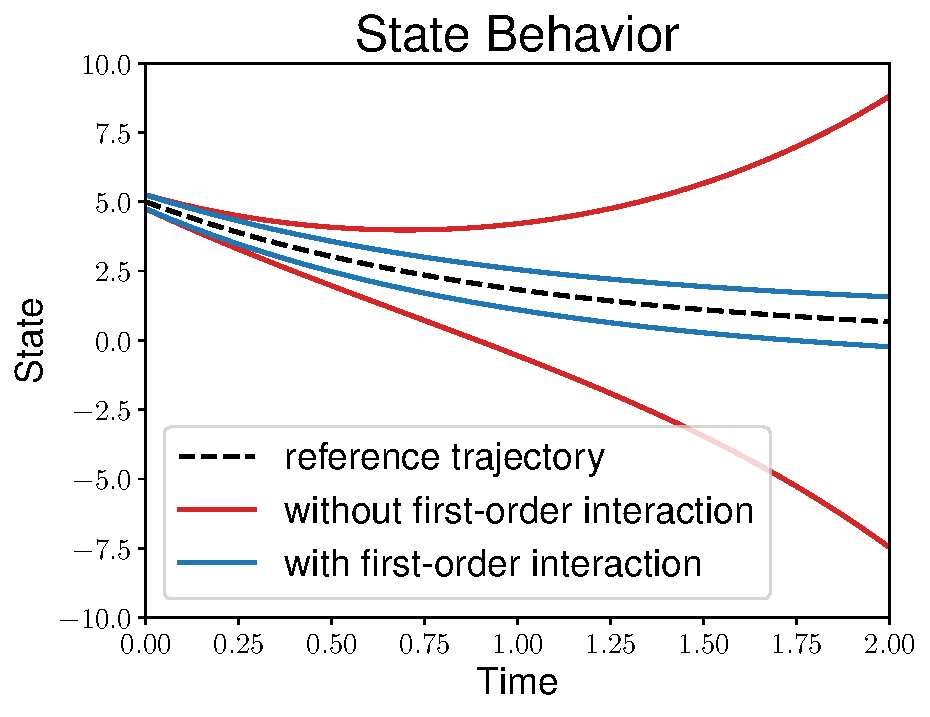
\includegraphics[width=0.7\linewidth]{fig/simplesystem.pdf}
    \caption{Demonstration of the advantages of including first-order interactions of the disturbance in the forward invariant tube calculation. By accounting for these interactions, the tube remains tight around the reference trajectory.}
    \label{fig:simple}
\end{figure}

We begin with a simple numerical example showcasing the effects of incorporating the first-order interactions of the observed disturbance behavior on the system. We consider the dynamics
\begin{equation}
    \dot{x} = x + u + w
\end{equation}
where the disturbance behavior $w = g(x)$ is dictated by the function $g(x) = -x$. We assume we have estimated disturbance bounds
\begin{align}
    \ul{\gamma}(t, \ul{x}, \ol{x}) &= \min_{x\in[\ul{x}, \ol{x}]}{-x - 1} \\
    \ol{\gamma}(t, \ul{x}, \ol{x}) &= \max_{x\in[\ul{x}, \ol{x}]}{-x + 1}
\end{align}
and known reference controller behavior $u_r = -x$ as well as feedback controller behavior $u = -(x - x_r) + u_r$. We initialize the system at $x = 5$ and then craft two embedding systems: one without modeling the first-order disturbance interactions (i.e.~\eqref{eq:initial_emb_bounds}), and one with them (i.e.~\eqref{eq:final_emb}). We initialize both embedding systems at $[x, \widehat{x}] = [4.75, 5.25]$ and simulate a $2$ second trajectory. As shown in Figure~\ref{fig:simple}, by accounting for the first-order interactions between the disturbance behavior and the system, the forward invariant tube remains tight around the reference trajectory, rather than quickly expanding.



\subsection{Trajectory Tracking Runtime Assurance}
\begin{figure}[t!]
\centering
  
  \begin{tikzpicture}
    \begin{axis}[width=1in,
    axis y line=middle,
    axis x line=middle,
every axis x label/.style={at={(current axis.right of origin)},anchor=west},
   xmin=0, xmax=2, ymax=1.5,ymin=0, ytick=\empty, xtick=\empty,xticklabel={$-\frac{b}{M}$}, yticklabel style={anchor=west},
   xlabel style={anchor=north},
   ylabel style={anchor=north east},
    xlabel={$y$},
    ylabel={$z$},
    x=1cm,y=1cm, 
    disabledatascaling,
    clip=false
    ]
    \addplot[mblue, line width=1pt] file {quad.txt};
    \draw[dashed] (0,0) -- +(20:1.8);
    \draw[->] (1.5,0) arc (0:20:1.5) node[right, pos=.5] {$\theta$};
    \draw[->, line width=1pt, draw=gray] (0,0) -- node[left,pos=1]{$u_1$}+(110:.8);
    \draw[->, line width=1pt, draw=gray] (20:.2) arc (20:310:.2) node[below,pos=.8] {$u_2$};
    \draw[->, dashed] (1.4,0.5) -- node[right,pos=1]{}+(20:.8);
    % \draw[->, dashed] (1.4,0.5) -- node[left,pos=1]{$v$}+(110:.8);
%    \node at (1.8,.7) {$(y,z)$};
  %  \node [circle, fill=blue, inner sep=1pt] at (1.3,1) {};
  \end{axis}

  \end{tikzpicture}
  \caption{The planar multirotor model has horizontal position $y$, vertical position $z$, and roll angle $\theta$. The inputs are thrust $u_1$ in the direction perpendicular to the line segment connecting the rotors and roll angle acceleration $u_2$.}
  \label{fig:quad}
\end{figure}

\begin{figure}
    \centering
    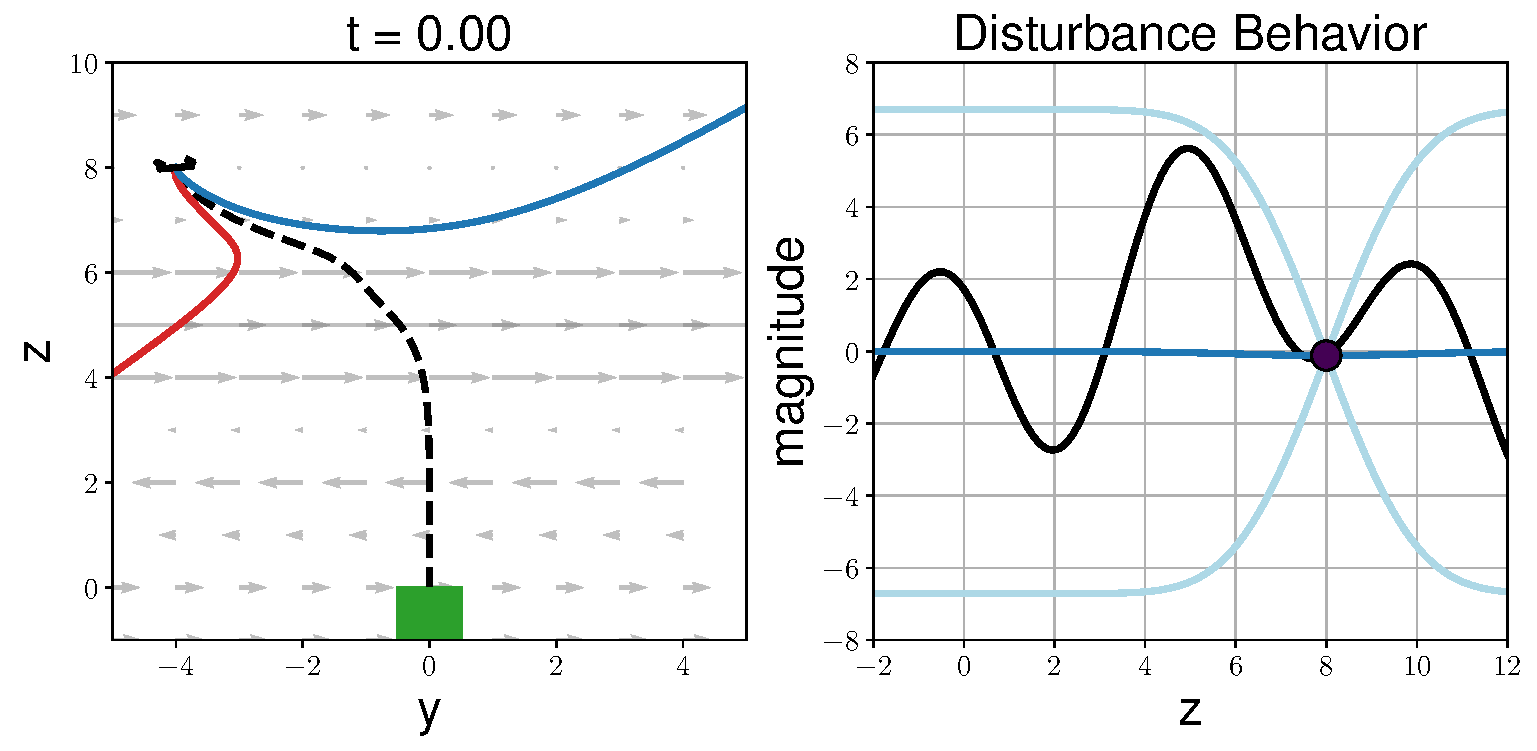
\includegraphics[width=0.9\linewidth]{fig/rta_0.00.pdf}
    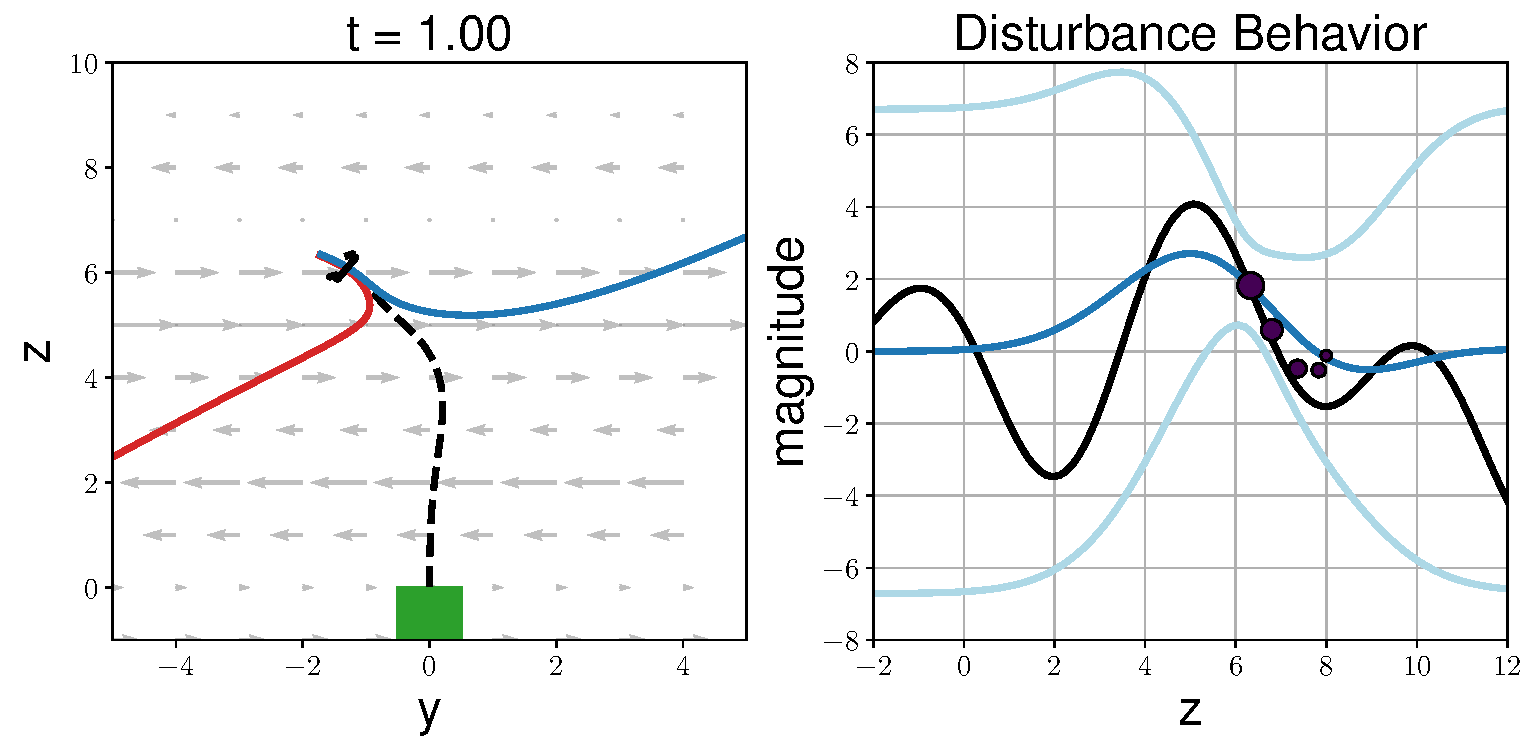
\includegraphics[width=0.9\linewidth]{fig/rta_1.00.pdf}
    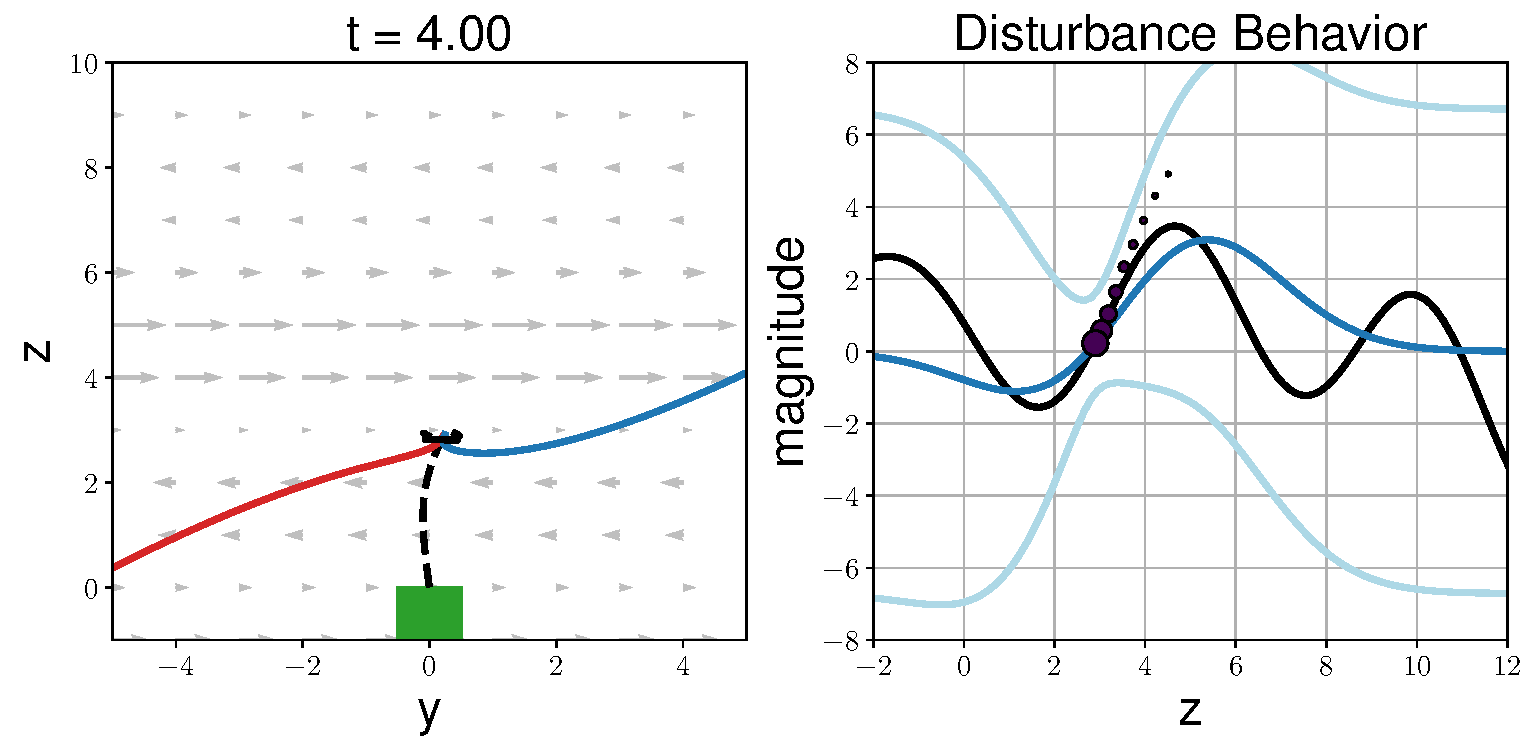
\includegraphics[width=0.9\linewidth]{fig/rta_4.00.pdf}
    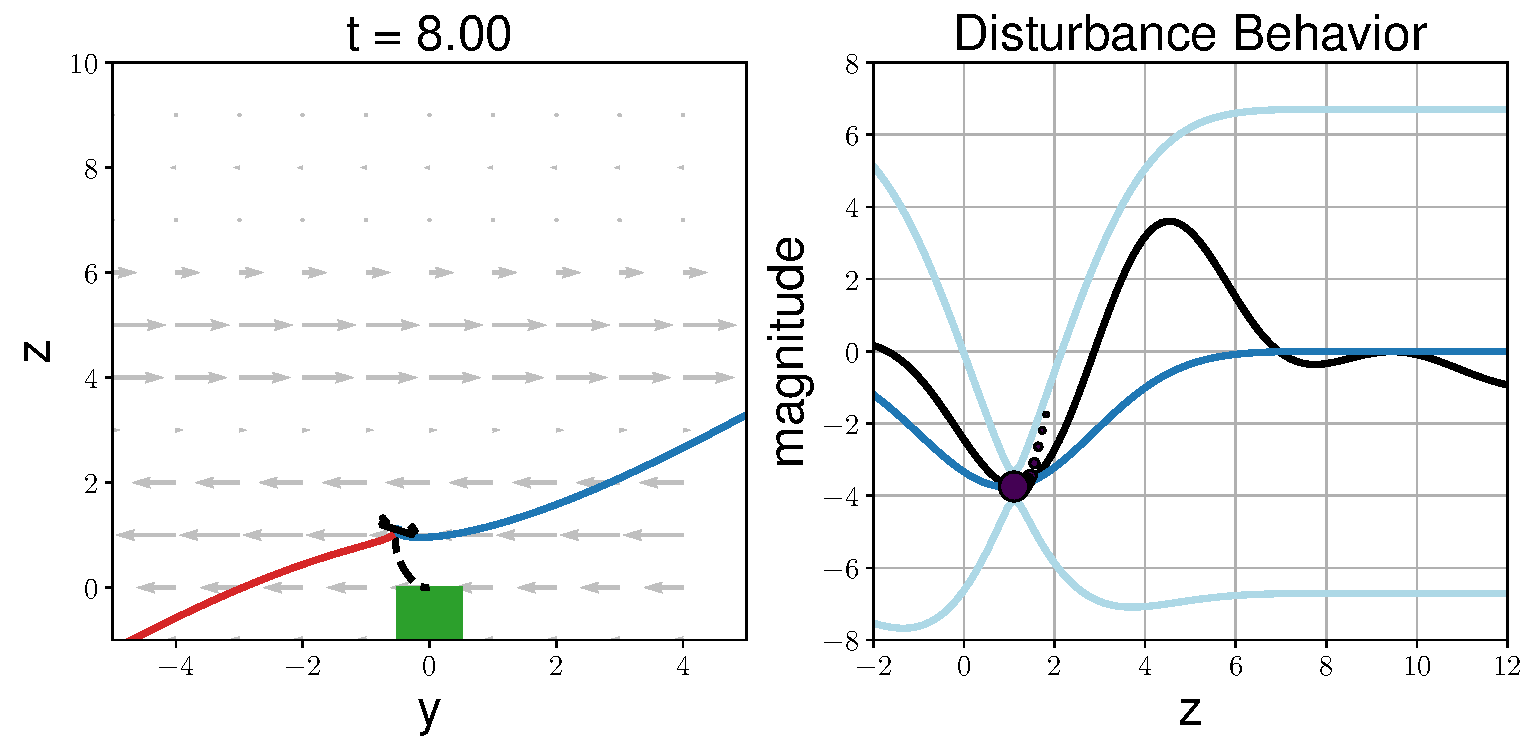
\includegraphics[width=0.9\linewidth]{fig/rta_8.00.pdf}
    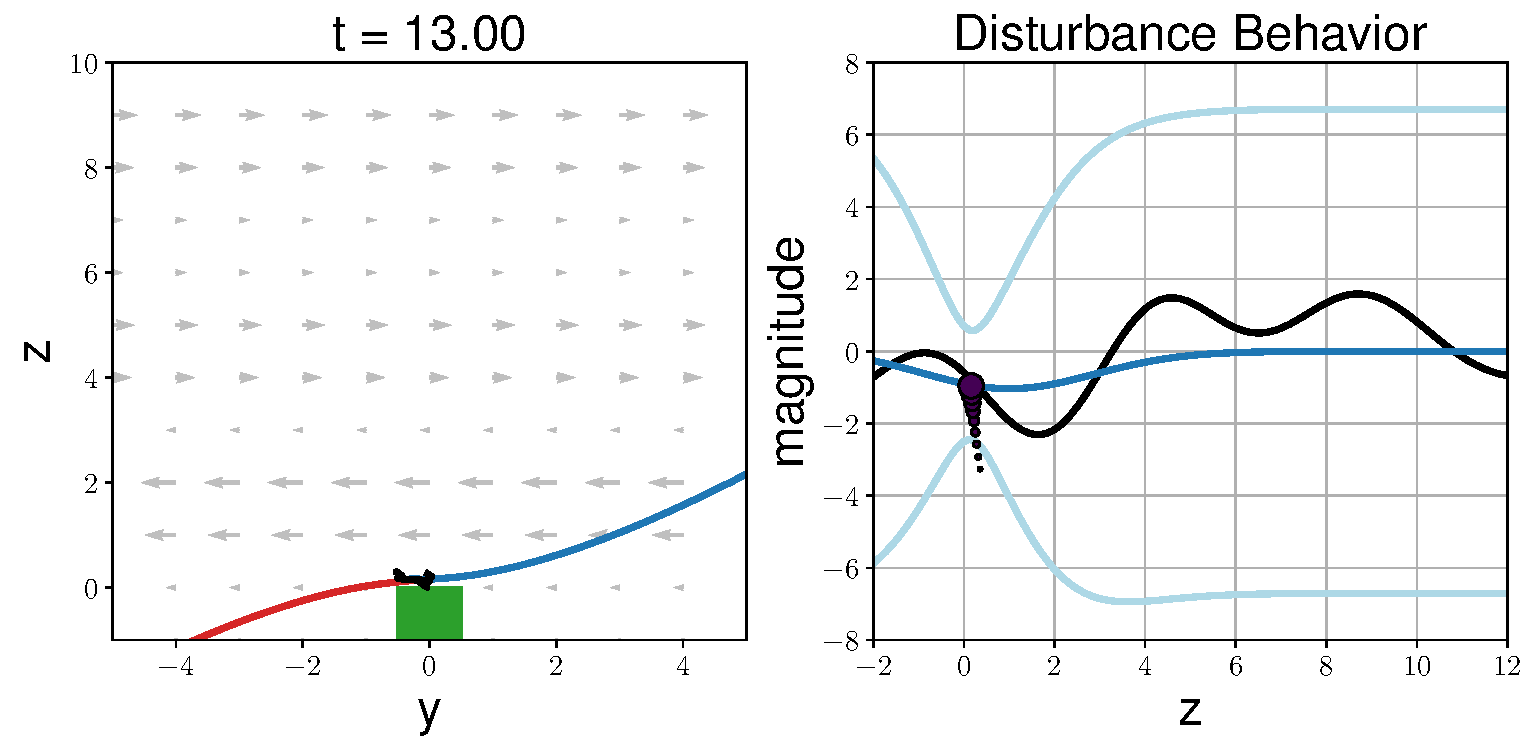
\includegraphics[width=0.9\linewidth]{fig/rta_13.00.pdf}
    \caption{The planar multirotor trajectory tracking simulation. The multirotor attempts to track a landing reference trajectory (left, dashed), while the runtime assurance algorithm calculates a forward invariant tube (left, red and blue) using observations (right, dots, largest most recent) to estimate the mean and confidence bounds (right, dark and light blue respectively) on the disturbance (right, solid black). Per Algorithm~\ref{alg:mechanism}, an observation is collected and the trajectories are recomputed whenever the forward invariant tube deviates from the reference beyond the safety threshold.}
    \label{fig:rta}
\end{figure}

We now consider a multirotor system constrained to moving within the vertical plane, and apply our forward invariant tube calculation to the runtime assurance mechanism outlined in~\cite{caoICRARTA}. The five-dimensional state $x$ of the planar multirotor system consists of horizontal position $y$, vertical position $z$, roll angle $\theta$, and the derivatives $\dot{y}$ and $\dot{z}$, so that $x=\begin{bmatrix}y\ \dot{y}\ z\ \dot{z}\ \theta\end{bmatrix}^T$. The two inputs are thrust $u_1$  acting at the center of mass in the direction $\begin{bmatrix}-\sin\theta&\cos\theta\end{bmatrix}^T$ perpendicular to the line segment connecting the rotors, and roll angular velocity $u_2$. Additionally, there exists a time and altitude-dependent wind force $g(t, z)$ acting horizontally which is unknown a priori. Thus, the normalized dynamics of the system are
\begin{equation}
  \label{eq:planarquad}
  \begin{split}
  \ddot{y}&=-u_1\sin \theta+g(t, z)\\
  \ddot{z}&=u_1\cos \theta-a_g\\
  \dot{\theta}&=u_2
  \end{split}
\end{equation}

We then implement the runtime assurance algorithm outlined in~\cite{caoICRARTA} and insert the forward invariant tube calculation~\eqref{eq:final_emb}. We first generate a reference trajectory by linearizing the system~\eqref{eq:planarquad} around the equilibrium and then employing a Linear-Quadratic Regulator (LQR) feedback controller with parameters
$Q = \text{diag}([1000, 500, 20, 500, 1])$ and $R = \text{diag}([20, 20])$ to simulate a trajectory to the origin assuming $g(t, z) = \widetilde{\mu}_t(z_r)$. The resulting state and input trajectories form the reference trajectories $x_r, u_r$ that we use to calculate the forward invariant tube.

We then designate a safe landing hyperrectangle $\mathcal{X}_\text{land} := [(-0.5, -0.1, -1, -0.1, -\pi/6), (-0.5, 0.1, 0, 0.1, \pi/6)]$ and then calculate the forward invariant tube of the system using the embedding system~\eqref{eq:final_emb} and the current estimated $\widetilde{\mu}_t, \widetilde{\sigma}_t$. We apply the control strategy~\eqref{eq:feedback_controller} and calculate the future time $t_r$ at which any state deviates beyond the reference trajectory by $\varepsilon$ or more. At that time, we collect an observation of the disturbance behavior and recalculate the reference trajectory and forward invariant tube. This guarantees that the system remains within $\varepsilon$ of the reference trajectory for all time. The overall runtime assurance mechanism is outlined in Algorithm~\ref{alg:mechanism}.

\begin{algorithm}
\caption{Runtime Assurance Mechanism}
\label{alg:mechanism}
\begin{algorithmic}[1]
\State\algorithmicKwData{Embedding system \eqref{eq:final_emb}, safety threshold $\varepsilon$, feedback coefficient matrix $K$}

\State$t_r \gets 0$
\While{In Operation}
\If{$t \geq t_r$}
\State Generate Reference Trajectories $x_r, u_r$ which solve~\eqref{eq:system} for $w_r = \widetilde{\mu}_t(x_r)$, $x_r(t) = x(t)$;
\State $\ul{x}, \ol{x} \gets$ solution to~\eqref{eq:final_emb}, $\ul{x}(t) = \ol{x}(t) = x(t)$;
\State $t_r \gets \min_{t \geq 0} |\ul{x}_i(t) - x_{ri}(t)| \geq \varepsilon \vee |\ol{x}_i(t) - x_{ri}(t)| \geq \varepsilon$;
\EndIf
\State Apply $u = K(x - x_r) + u_r$;
\EndWhile

\end{algorithmic}
\end{algorithm}



As shown in Figure~\ref{fig:rta}, the multirotor is initially unable to guarantee a safe landing as the forward invariant tube quickly expands past the allowed threshold. As the quadcopter descends, we collect observations and update the reference trajectory and forward invariant tube, taking into account the time at which each observation was taken and weighting them appropriately in the confidence bounds on the disturbance behavior. The multirotor is eventually able to achieve a safe landing even in the presence of this time-varying disturbance behavior. We implement this simulation on a personal computer with the \texttt{immrax} library~\cite{immrax}. Calculating the reference trajectories and the forward invariant tube takes approximately $0.04$ seconds, and a recalculation is triggered approximately every $0.3$-$1.0$ seconds, showcasing the real-time capabilities of the formulation.

\subsection{Implicit Active Set Invariance Filtering}
\begin{figure}
    \centering
    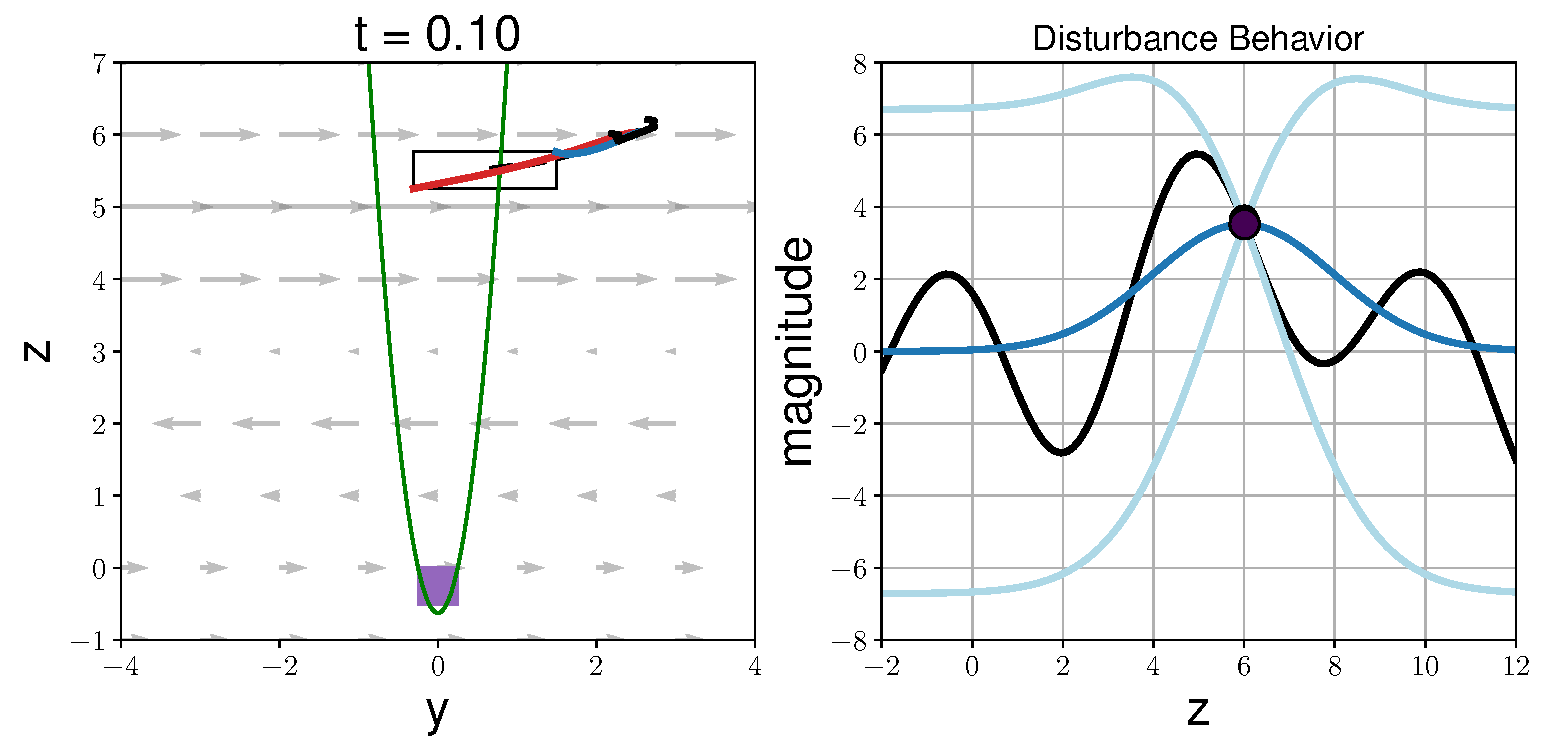
\includegraphics[width=0.9\linewidth]{fig/iasif_0.10.pdf}
    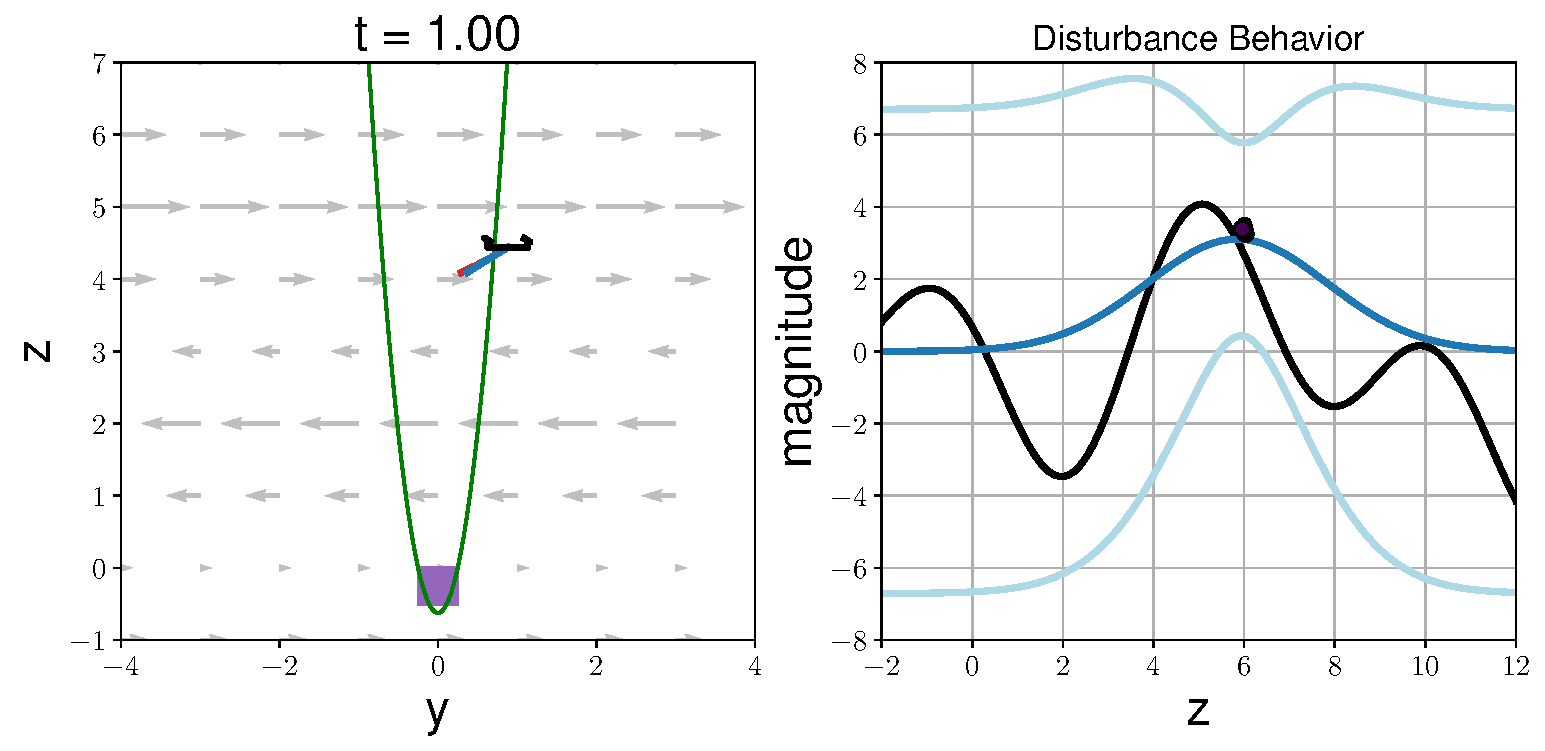
\includegraphics[width=0.9\linewidth]{fig/iasif_1.00.pdf}
    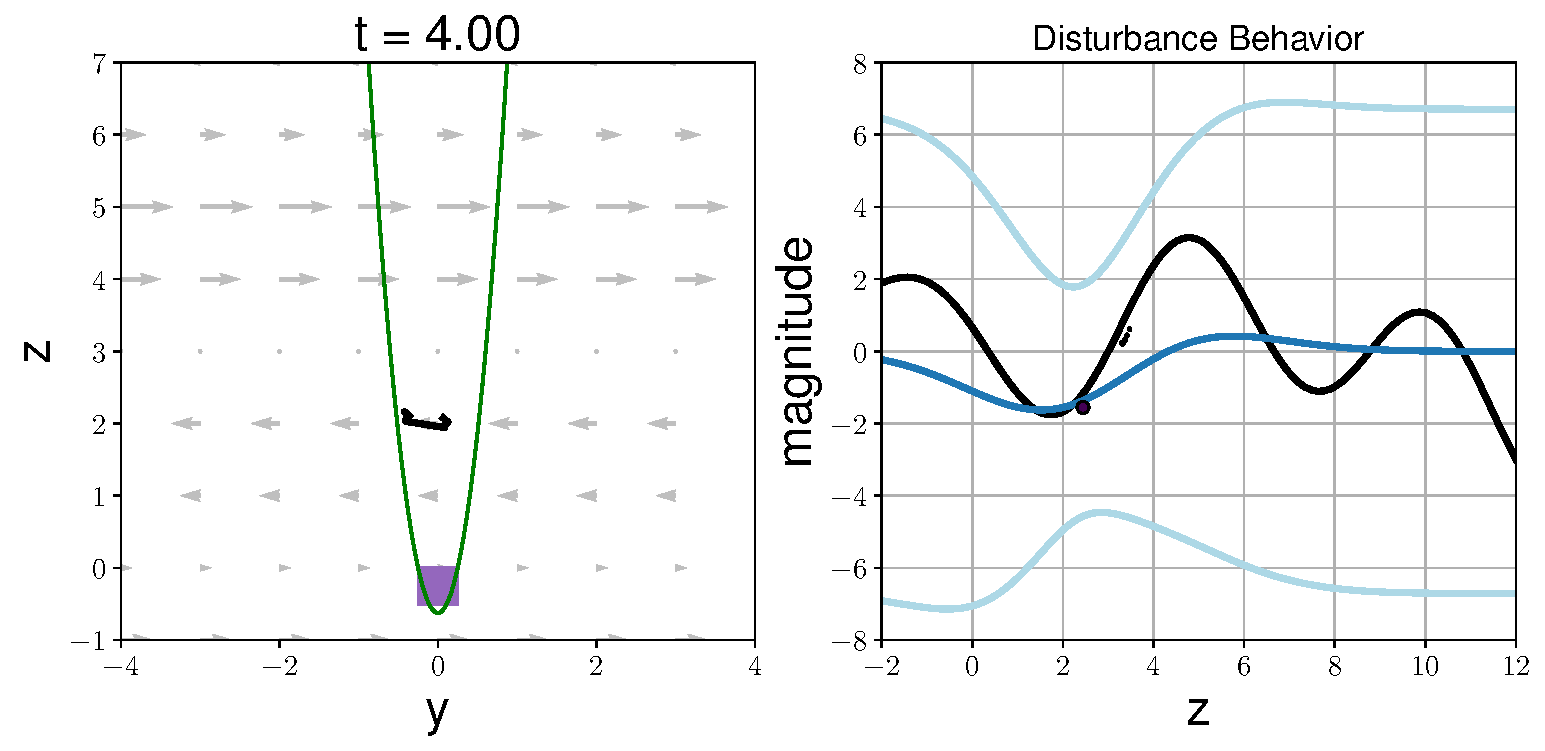
\includegraphics[width=0.9\linewidth]{fig/iasif_4.00.pdf}
    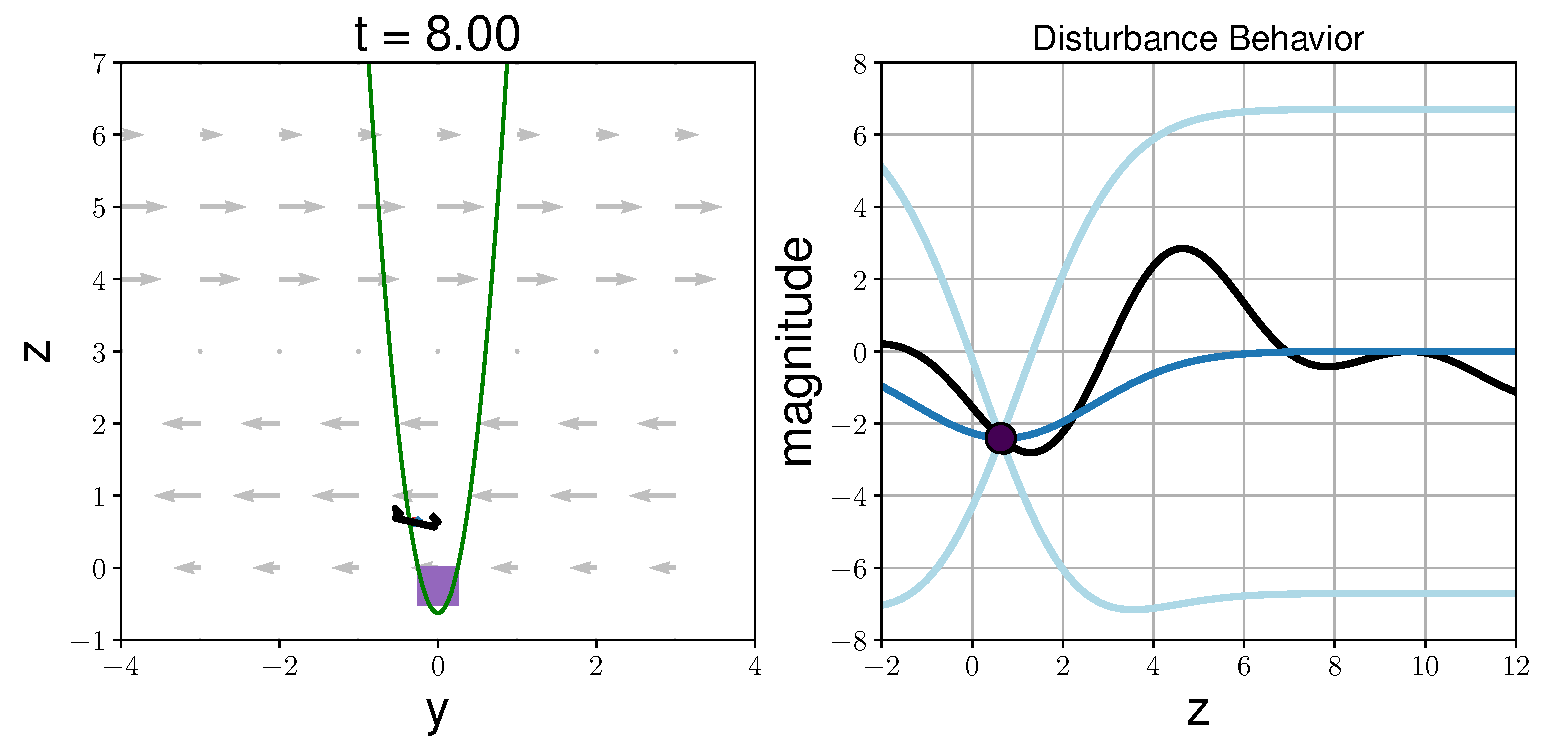
\includegraphics[width=0.9\linewidth]{fig/iasif_8.00.pdf}
    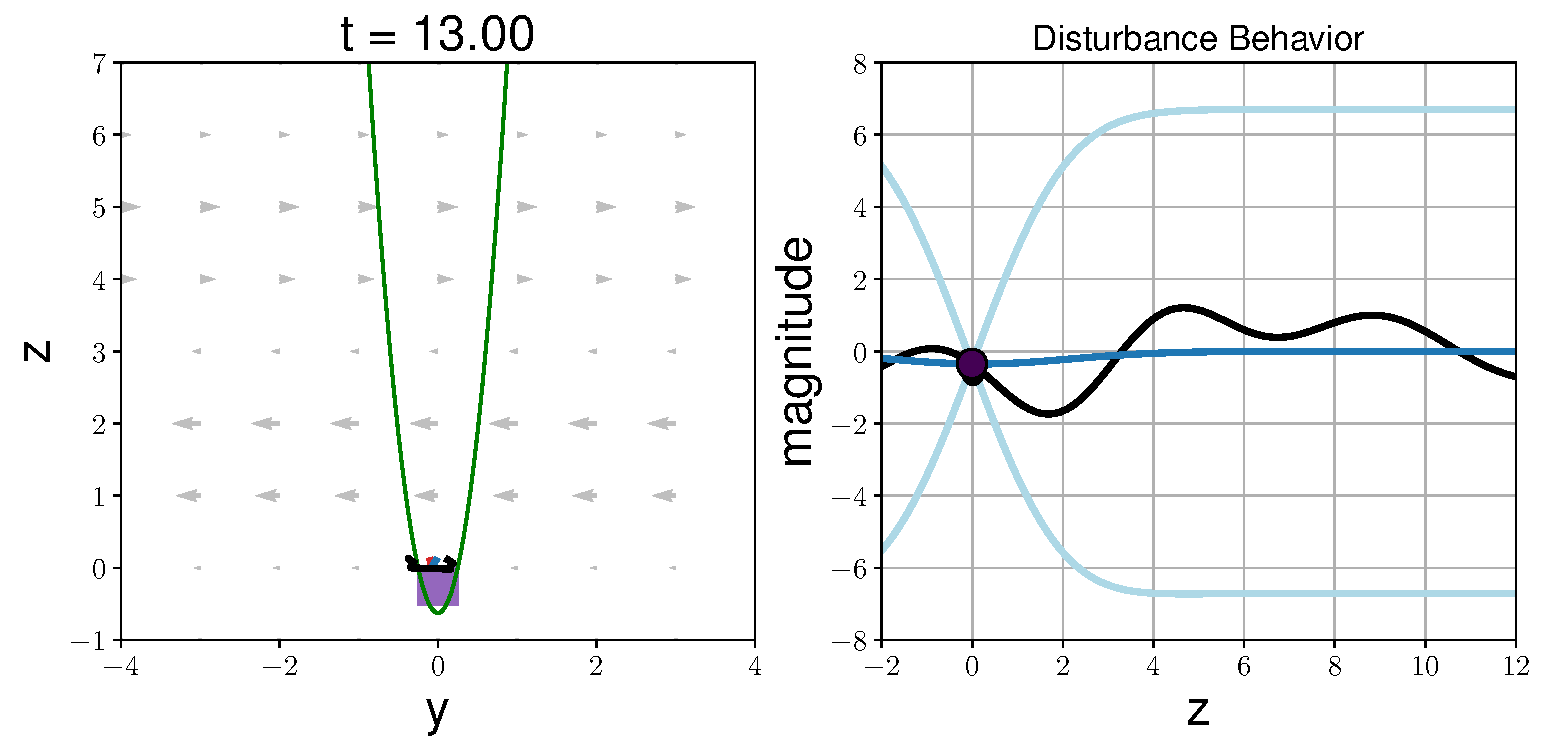
\includegraphics[width=0.9\linewidth]{fig/iasif_13.00.pdf}
    \caption{The planar multirotor Implicit ASIF simulation. The multirotor attempts to land via an uncertified controller. At all times, the filter calculates the least intrusive modification to the desired input such that a backup trajectory (left, red and blue) back to the safety region (left, green) always exists. The formulation incorporates observations (right, dots, largest most recent) to estimate the mean and confidence bounds (right, dark and light blue respectively) on the disturbance (right, solid black), which are collected whenever no part of the forward invariant tube fully fits within the safety region.}
    \label{fig:iasif}
\end{figure}

We now consider a scenario in which a separate, unverified control strategy is developed for landing, and insert our trajectory tracking formulation into an Implicit Active Set Invariance Filtering formulation to act as a safety filter for said controller. We define a function $h(x)$ and a resulting safety set $\mathcal{S}$ such that
\begin{equation}
    \mathcal{S}:= \{x \in \mathbb{R}^n | h(x) \geq 0\},
\end{equation}
which, for this case study, is defined as
\begin{equation}
    h(x) := -(10(y^2 - 0.0625) - z)
\end{equation}
which produces the region outlined in green in Figure~\ref{fig:iasif}.

We then implement an Implicit Active Set Invariance Filter (see, e.g.,~\cite{llanesIASIF}), which minimally perturbs the desired input such that a backup trajectory that drives the system into $\mathcal{S}$ always exists. Our embedding system formulation~\eqref{eq:final_emb} produces the backup trajectory and forward invariant tube used in the filter. As shown in Figure~\ref{fig:iasif}, when there is no guaranteed path back to the safety set (i.e., no slice of the forward invariant tube is fully contained in the safety set), an observation is taken and the filter steps in and drives the system with the maximum force back toward it. This continues until a safe landing is achieved. The filter takes around $0.01$ seconds to compute on average, showcasing its capabilities for real-time computation.

\subsection{Hardware Demonstration}
TBD

\section{Conclusion}
\label{section:conclusion}
We presented a general interval mixed-Jacobian-based formulation for efficiently computing a forward invariant tube around a reference trajectory for nonlinear systems subject to time- and state-dependent disturbance behaviors. By collecting time-weighted observations and modeling the disturbance behavior as a \ac{GP}, the formulation produces a forward invariant tube which holds with high probability. Additionally, we incorporate the first-order interactions between the feedback controller, disturbance behavior, and the system state, resulting in a tighter approximation. This formulation is fast enough to be used in direct trajectory tracking and as part of an implicit active set invariance filter, and is demonstrated on hardware.

\addtolength{\textheight}{-12cm}   % This command serves to balance the column lengths
                                  % on the last page of the document manually. It shortens
                                  % the textheight of the last page by a suitable amount.
                                  % This command does not take effect until the next page
                                  % so it should come on the page before the last. Make
                                  % sure that you do not shorten the textheight too much.


\bibliographystyle{plain}
\bibliography{ref}



\end{document}
